 
\iffalse
\chapter{2015}
\author{Prajwal naik}
\section{me}
\fi












    \item  Choose the appropriate word phrase, out of the four options given below, to complete the following sentence:\\
    Dhoni, as well as the other team members of Indian team,\rule{1cm}{0.15mm} present on the occassion.
    \hfill{\brak{2015}}
    \begin{multicols}{4}
        
    
\begin{enumerate}
    \item were 
    \item was
    \item has
    \item have
\end{enumerate}
   \end{multicols}
        
  \item   Choose the word most similar in meaning to the given word:\\Awkward
   \hfill{\brak{2015}}
  \begin{multicols}{4}
    \begin{enumerate}
        \item Inept 
        \item Graceful
        \item Suitable
        \item Dreadful
    \end{enumerate}  
  \end{multicols}

 
  
  \item What is the adverb for the given word below?

\textbf{Misogynous}\\
 \hfill{\brak{2015}}
\begin{multicols}{4}
    \begin{enumerate}
        \item   Misogynousness
        \item Misogynity
        \item  Misogynously
        \item Misogynous
    \end{enumerate}
\end{multicols}
\item An electric bus has onboard instruments that report the total electricity consumed since the start of the trip as well as the total distance covered. During a single day of operation, the bus travels on stretches ${M}, {N}, {O}$, and P , in that order. The cumulative distances travelled and the corresponding electricity consumption are shown in the Table below:
    \begin{tabular}{|c|c|c|}
\hline Stretch & Cumulative distance (km) & Electricity used (kWh) \\
\hline M & 20 & 12 \\
\hline N & 45 & 25 \\
\hline O & 75 & 45 \\
\hline P & 100 & 57 \\
\hline
\end{tabular}\\
    The stretch where the electricity consumption per km is minimum is
     \hfill{\brak{2015}}
\begin{multicols}{4}
    \begin{enumerate}
        \item M
        \item N
        \item O
        \item P
    \end{enumerate}
\end{multicols}
  
  \item Ram and Ramesh appeared in an interview for two vacancies in the same department. The probability of Ram's selection is $\frac{1} { 6}$ and that of Ramesh is $\frac{1} { 8}$. What is the probability that only one of them will be selected?
  \hfill{\brak{2015}}
  \begin{multicols}{4}
			\begin{enumerate}
   \item $\frac{47}{48}$
\item $\frac{1}{4}$
\item $\frac{13}{48}$
\item  $\frac{35}{48}$
\end{enumerate}
		\end{multicols}
   
%33
\item In the following sentence certain parts are underlined and marked $P, Q$, and $R$. One of the parts may contain certain error or may not be acceptable in standard written communication. Select the part containing an error. Choose D as your answer if there is no error.\\
The student corrected all the errors that the instructor marked on the answer book.
 \hfill{\brak{2015}}
   \begin{multicols}{4}
			\begin{enumerate}
   \item P
\item  Q
\item Q
\item  No Error
\end{enumerate}
		\end{multicols}
  \item  Given below are two statements followed by two conclusions. Assuming these statements to be true, decide which one logically follows.
  

Statements:
I. All film stars are playback singers.
II. All film directors are film stars.

\textbf{Conclusions:}\
I. All film directors are playback singers.
II. Some film stars are film directors.
 \hfill{\brak{2015}}
\begin{enumerate}
    
\item  Only conclusion I follows.
  \item  Only conclusion II follows.
\item  Neither conclusion I nor II follows.
 \item  Both conclusions I and II follow.
\end{enumerate}

  \item   A tiger is 50 leaps of its own behind a deer. The tiger takes 5 leaps per minute to the deer's 4 . If the tiger and the deer cover 8 metre and 5metre per leap respectively, what distance in metres will the tiger have to run before it catches the deer?
  \hfill{\brak{2015}}
 \item If $a^{2}+b^{2}+c^{2}=1$, then $a b+b c+a c$ lies in the interval
 \hfill{\brak{2015}}
  \begin{multicols}{4}
      
  
  \begin{enumerate}
    \item $[1,2 / 3]$
    \item $[-1 / 2,1]$
    \item  $[-1,1 / 2]$
  \end{enumerate}
  \end{multicols}
  
\item Lamenting the gradual sidelining of the arts in school curricula, a group of prominent artists wrote to the Chief Minister last year, asking him to allocate more funds to support arts education in schools. However, no such increase has been announced in this year's Budget. The artists expressed their deep anguish at their request not being approved, but many of them remain optimistic about funding in the future.
Which of the statement(s) below is/are logically valid and can be inferred from the above statements?

(i) The artists expected funding for the arts to increase this year.\\
(ii) The Chief Minister was receptive to the idea of increasing funding for the arts.\\
(iii) The Chief Minister is a prominent artist.\\
(iv) Schools are giving less importance to arts education nowadays.
 \hfill{\brak{2015}}

			\begin{enumerate}
\item  (iii) and (iv)
\item (i) and (iv)
\item (i), (ii) and (iv)
\item (i) and (iii)
   \end{enumerate}

  \item If any two columns of determinant  of matrix $A =\myvec{4 & 7 & 8\\ 3 & 1 & 5\\ 9 & 6 & 2}$ are interchanged , which of the following statements regarding the value of the determinant is CORRECT?
   \hfill{\brak{2015}}
\begin{enumerate}
    \item Absolute value remains unchanged but sign will change
    \item Both absolute value and sign will change
    \item Absolute value will change but sign will not change
    \item Both absolute value and sign will remain unchanged
\end{enumerate}

  \item Among the four normal distributions with probability density functions as shown below , which one has the lowest variance
  \begin{figure}[h!]
    \centering
    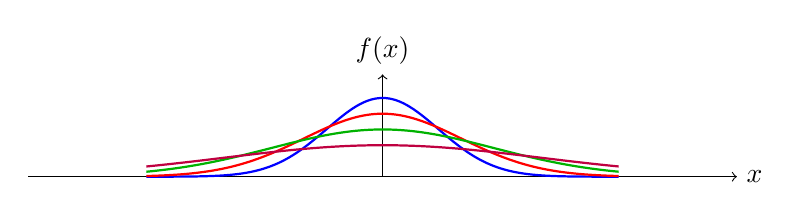
\begin{tikzpicture}
    % Draw the x and y axes
    \draw[->] (-4.5, 0) -- (4.5, 0) node[right] {$x$};
    \draw[->] (0, 0) -- (0, 1.3) node[above] {$f(x)$};

    % First normal distribution (narrowest)
    \draw[thick, blue, smooth, domain=-3:3, samples=100] 
        plot ({\x}, {exp(-\x*\x)}) node[pos=0.50, right] {};

    % Second normal distribution (wider)
    \draw[thick, red, smooth, domain=-3:3, samples=100] 
        plot ({\x}, {0.8*exp(-0.5*\x*\x)}) node[pos=0.95, right] {};

    % Third normal distribution (even wider)
    \draw[thick, green!70!black, smooth, domain=-3:3, samples=100] 
        plot ({\x}, {0.6*exp(-0.25*\x*\x)}) node[pos=0.95, right] {};

    % Fourth normal distribution (widest)
    \draw[thick, purple, smooth, domain=-3:3, samples=100] 
        plot ({\x}, {0.4*exp(-0.125*\x*\x)}) node[pos=0.95, right] {} ;
\end{tikzpicture}
\end{figure}

   \hfill{\brak{2015}}
  
\begin{enumerate}
    \item I(Blue)
    \item II(Red)
    \item III(Green)
    \item IV(Pink)
\end{enumerate}

\item Simpson's $\frac{1}{3}$ rule is used to integrate the function $f(x)=\frac{3}{5}x^2+\frac{9}{5}$ between $x=0$ and $x=1$ using the least number of sub-intervals . The value of the integral is .
 \hfill{\brak{2015}}





